% ------------------------------------------------------------------------------
%						3 Conclusion
% ------------------------------------------------------------------------------
\section{Conclusion}
\label{sect:conclusion}

The cluster operates on a ``first-come, first-served'' basis until it reaches full capacity.
After that, job positions in the queue are determined based on past usage.
The scheduler does attempt to fill gaps, so occasionally, a single-core job with lower priority
may be scheduled before a multi-core job with higher priority.

% 3.1 Important Limitations
% -------------------------------------------------------------
\subsection{Important Limitations}
\label{sect:limitations}

While Speed is a powerful tool, it is essential to recognize its limitations to use it effectively:

\begin{itemize}
	\item New users are limited to a total of 32 cores and 4 GPUs. If you need more cores temporarily,
	please contact \texttt{rt-ex-hpc AT encs.concordia.ca}.

	\item Batch job sessions can run for a maximum of one week.
	Interactive jobs are limited to 24 hours see \xs{sect:interactive-jobs}.

	\item Scripts can live in your NFS-provided home directory, but substantial data should be stored in
    your cluster-specific directory (located at \verb+/speed-scratch/<USER>/+).
    NFS is suitable for short-term activities but not for long-term operations.
	Data that a job will read multiple times should be copied at the start to the scratch disk of a compute node using
	\api{\$TMPDIR} (and possibly \api{\$SLURM\_SUBMIT\_DIR}).
	Intermediate job data should be produced in \api{\$TMPDIR}, and once a job is near completion,
	these data should be copied to your NFS-mounted home directory (or other NFS-mounted space).
	\textbf{In other words}, IO-intensive operations should be performed locally whenever possible,
	reserving network activity for the start and end of jobs.

	\item Your current resource allocation is based on past usage, which considers approximately
    one week's worth of past wall clock time (time spent on the node(s)) and compute activity (on the node(s)).

	\item Jobs must always be run within the scheduler's system. Repeat offenders who
	run jobs outside the scheduler risk losing cluster access.
\end{itemize}

% 3.2 Tips/Tricks
% -------------------------------------------------------------
\subsection{Tips/Tricks}
\label{sect:tips}

\begin{itemize}
	\item
	Ensure that files and scripts have Linux line breaks.
	Use the \tool{file} command to verify and \tool{dos2unix} to convert if necessary.

	\item
	Use \tool{rsync} (preferred over \tool{scp}) for copying or moving large amounts of data.

	\item
	Before transferring a large number of files between NFS-mounted storage and
	the cluster, compress the files into a \tool{tar} archive.

	\item
	If you plan to use a different shell (e.g., \tool{bash}~\cite{aosa-book-vol1-bash}),
	change the shell declaration at the beginning of your script(s).

	\item
	Request resources (cores, memory, GPUs) that closely match the actual needs of your job.
	Requesting significantly more than necessary can make your job harder to schedule when
	resources are limited. Always check the efficiency of your job with either \tool{seff}
	and/or the \option{--mail-type=ALL}, to adjust your job parameters.

	\item
	For any concerns or questions, email \texttt{rt-ex-hpc AT encs.concordia.ca}
\end{itemize}

% 3.3 Use Cases
% -------------------------------------------------------------
\subsection{Use Cases}
\label{sect:cases}

\begin{itemize}
	\item HPC Committee's initial batch about 6 students (end of 2019):
	\begin{itemize}
		\item 10000 iterations job in Fluent finished in $<26$ hours vs. 46 hours in Calcul Quebec
	\end{itemize}

	\item NAG's MAC spoofer analyzer~\cite{mac-spoofer-analyzer-intro-c3s2e2014,mac-spoofer-analyzer-detail-fps2014},
	such as \url{https://github.com/smokhov/atsm/tree/master/examples/flucid}
	\begin{itemize}
		\item compilation of forensic computing reasoning cases about false or true positives of hardware address spoofing in the labs
	\end{itemize}

	\item S4 LAB/GIPSY R\&D Group's:
	\begin{itemize}
		\item MARFCAT and MARFPCAT (OSS signal processing and machine learning tools for
		vulnerable and weak code analysis and network packet capture
		analysis)~\cite{marfcat-nlp-ai2014,marfcat-sate2010-nist,fingerprinting-mal-traffic}
		\item Web service data conversion and analysis
		\item {\flucid} encoders (translation of large log data into {\flucid}~\cite{mokhov-phd-thesis-2013} for forensic analysis)
		\item Genomic alignment exercises
	\end{itemize}

	\item \textbf{Concordia Virtual Tour++}, ConUHacks; by
    Chul Bin (Ben) Yoon, Computer Science;
    Mathys Loiselle, Computer Science, minor in Math and Stats;
    Denis Oh, Software Engineering;
    Ricardo Raji Chahine, Computer Science.
    \textbf{Project description:}
    \textit{Concordia Virtual Tour++} aims to improve Concordia's current virtual tour web page,
    which only features a single 360-degree image fixed in one spot. On the other hand, our project
    lets users move freely within the scene, much like a video game.
    3D Gaussian Splatting is a computer graphics technique that transforms real-world spaces into interactive 3D environments.
    The process begins by capturing multiple photographs of a space from different angles. Using these images,
    the system can reconstruct intermediate viewpoints and create a fully navigable 3D environment—similar to a video game,
    but representing an actual physical space.

    GitHub: \url{https://github.com/matlois75/ConUHacks_2025}

    Website: \url{https://conuhacks-2025-the-frogs.onrender.com/}

    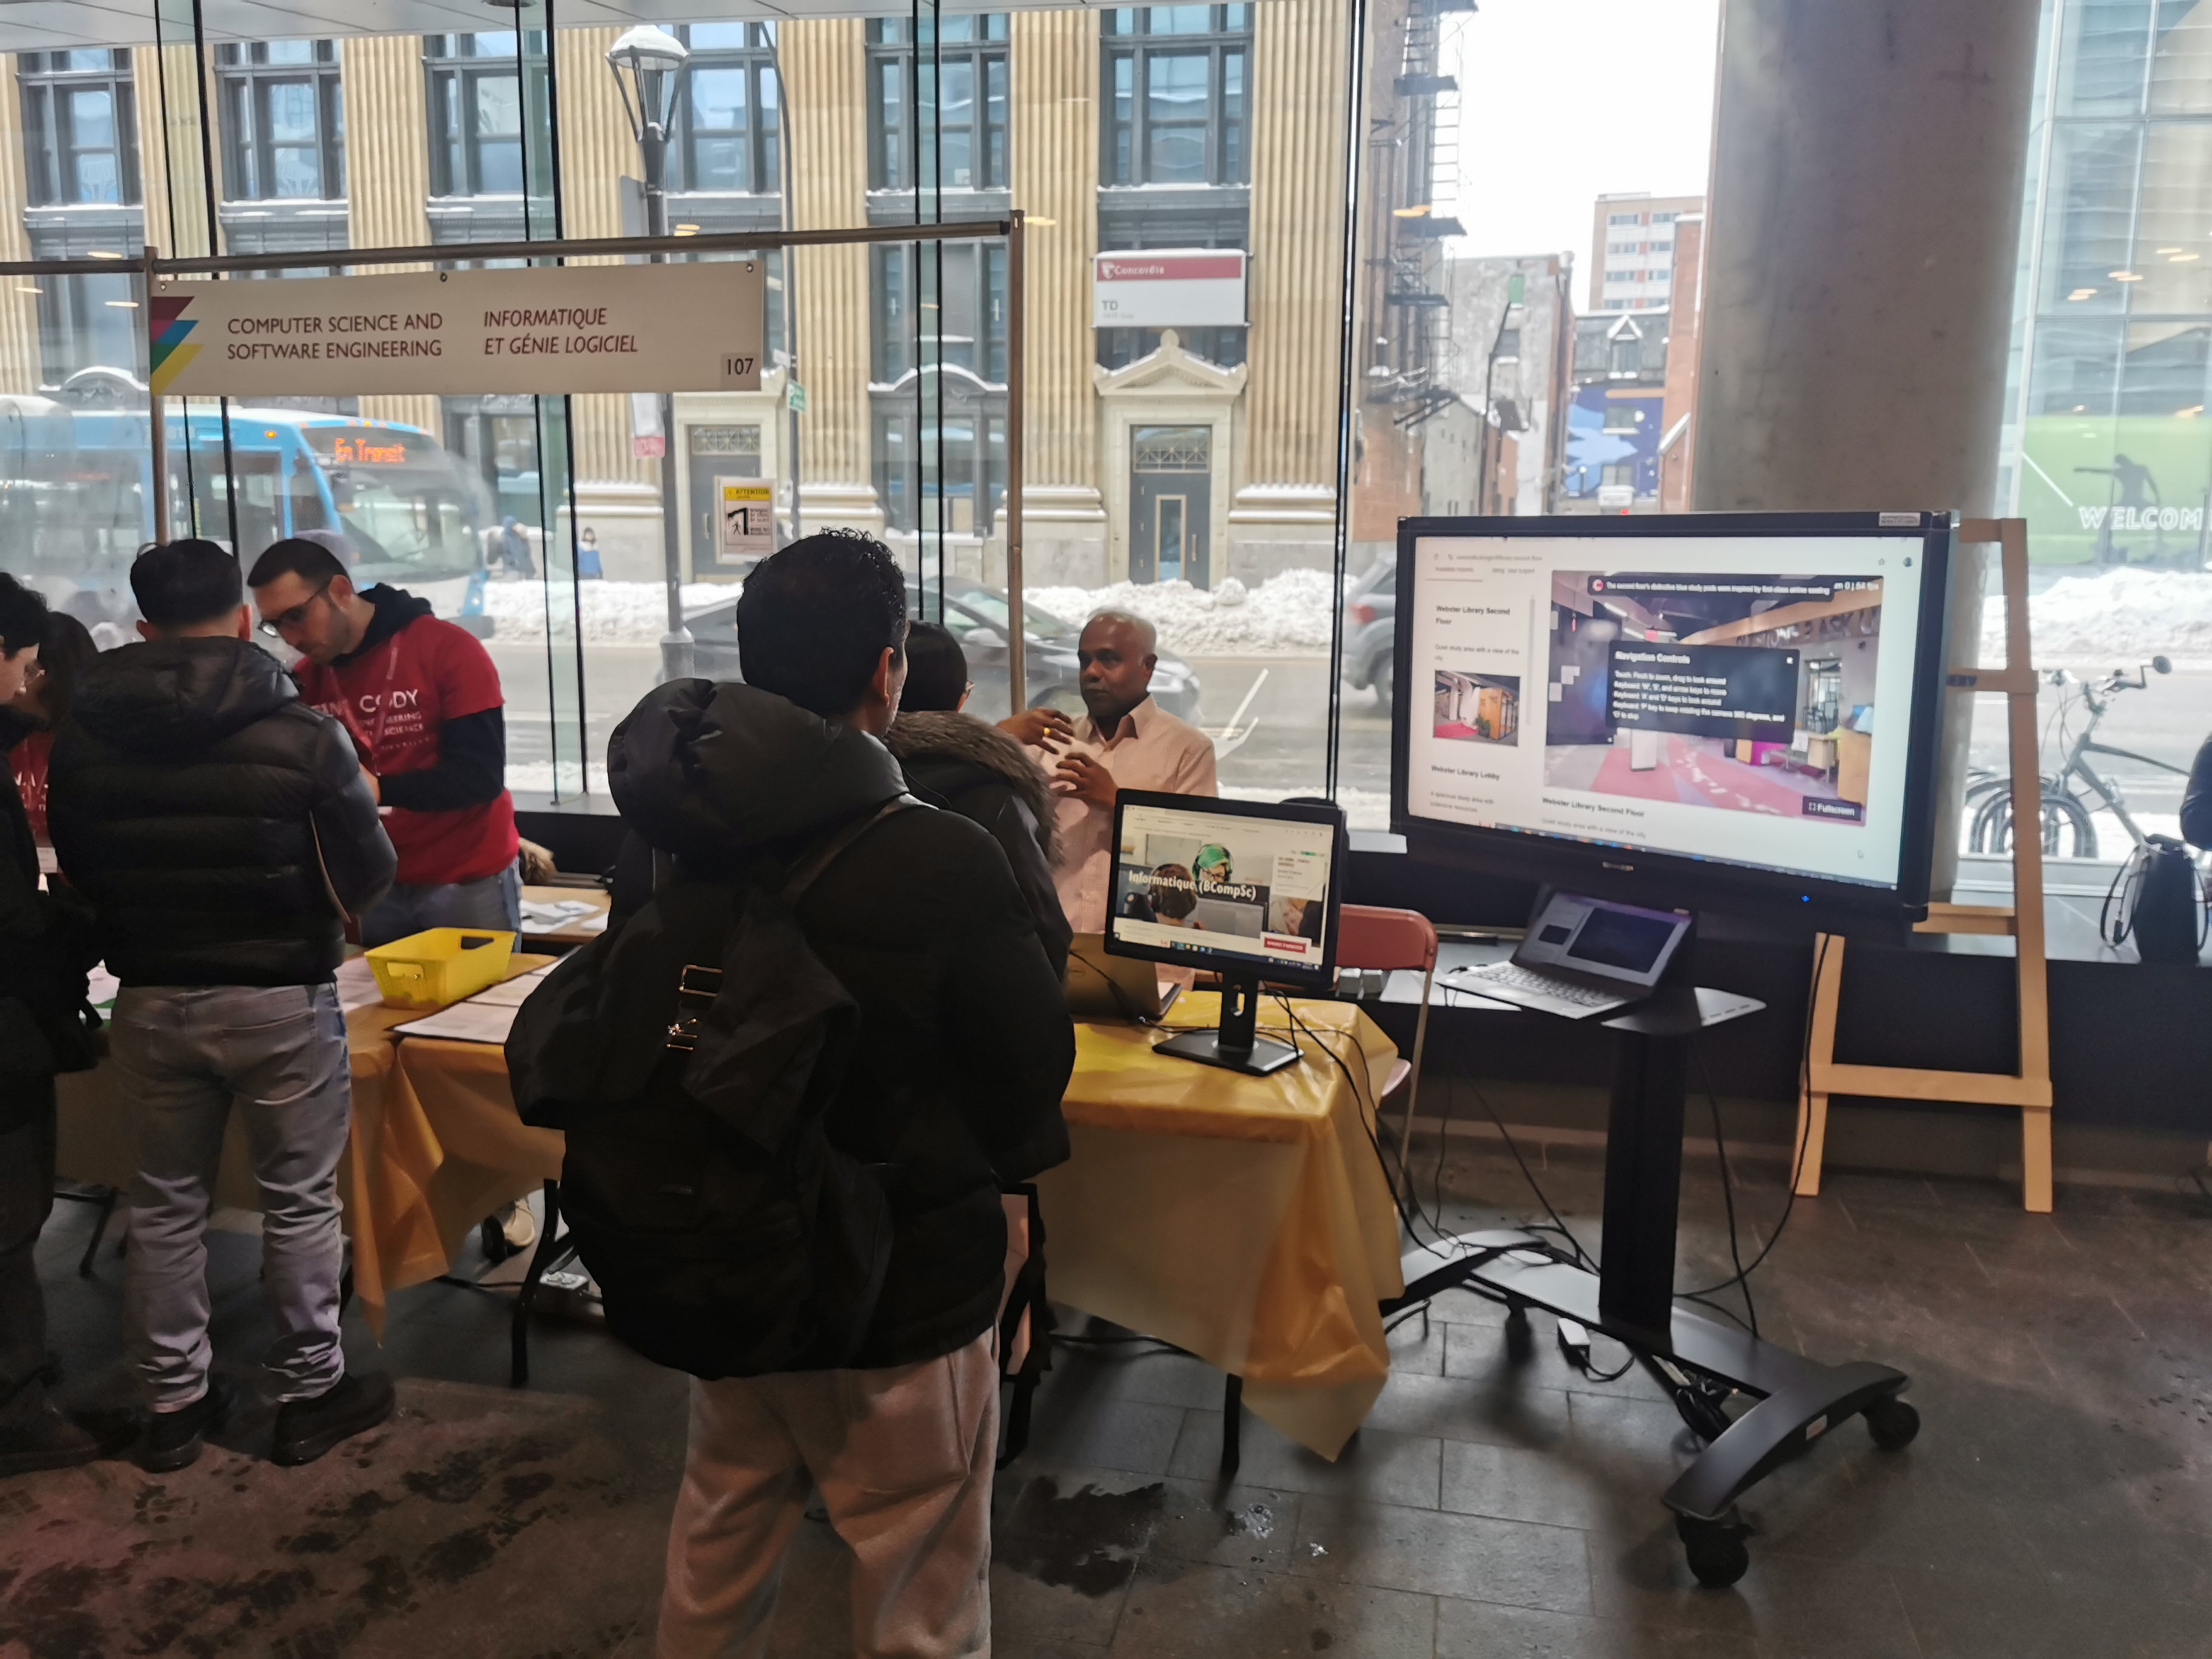
\includegraphics[width=\columnwidth]{images/gaussian-splatting-conu-open-house.jpg}

	\item \textbf{Best Paper award}, \bibentry{job-failure-prediction-compsysarch2024}
	\small
	% RT521027
	\item \bibentry{unsteady-wake-ouedraogo_essel_2023}
    \item \bibentry{effects-reynolds-ouedraogo_essel_2024}
    \item \bibentry{nozzle-effects-APS_2024}
	\item \bibentry{effects-reynolds-APS-ouedraogo_essel_2024}
	\item \bibentry{oi-containers-poster-siggraph2023}
	\item \bibentry{Gopal2024Sep}
	\item \bibentry{Gopal2023Mob}
	% the next one is not visible (it produces an error)
	%\item \bibentry{roof-mounted-vawt-2023}
	\item \bibentry{root-mounted-vawt-corner-2023}
	\item \bibentry{cfd-modeling-turbine-2023}
	\item \bibentry{small-vaxis-turbine-corner-2022}
	\item \bibentry{cfd-vaxis-turbine-wake-2022}
	\item \bibentry{numerical-turbulence-vawt-2021}
	\item \bibentry{niksirat2020}
	\item The work ``\bibentry{lai-haotao-mcthesis19}'' using TensorFlow and Keras on OpenISS adjusted to run on
    Speed based on the repositories, and theirs forks by the team:
	\begin{itemize}
		\item \bibentry{openiss-reid-tfk} and
		\item \bibentry{openiss-yolov3}
	\end{itemize}
	\normalsize
\end{itemize}